\documentclass[conference]{IEEEtran}
\usepackage{amsmath,amssymb}
\usepackage{booktabs}
\usepackage{graphicx}
\usepackage{tikz}
\usetikzlibrary{arrows.meta,positioning}
\usepackage{url}
\usepackage[hidelinks]{hyperref}

\graphicspath{{../results/figures/}}
\newcommand{\us}{\,\ensuremath{\mu}s}
\newcommand{\ba}{\ensuremath{g_a}}

\begin{document}

\title{AUTHBC: Feasibility Boundaries for Authenticated UAV Telemetry ---
An Exclusion Bound, a Capacity Envelope, and Hardware Validation}

\author{\IEEEauthorblockN{Mohamed A. Farouk}
\IEEEauthorblockA{AUTHBC Project --- Thesis draft (auto-generated from frozen results)}}

\maketitle

\begin{abstract}
Flying ad-hoc networks stream telemetry records so small that a cryptographic signature
(64--96\,B) rivals or exceeds the payload (45--190\,B), so per-record signing spends airtime,
energy and goodput on a shared, lossy channel. The operational question is not how many bytes a
scheme saves but \emph{which configurations can run at all}. We answer it by searching four design
choices jointly---record \emph{encoding}, authentication \emph{placement}, signature \emph{scheme}
and \emph{batch} size---against a byte model, an NS-3-validated 802.11 broadcast model, and energy
measured on Raspberry~Pi~4 hardware.

Three results follow, ordered by how durable they are. \textbf{An exclusion:} a link whose payload
cannot hold one header, one signature and one record carries no per-frame-verifiable telemetry at
\emph{any} encoding or batch size. This removes the four longest-range LoRa modes outright, and loss
makes fragmentation no escape, since a unit spanning $n$ frames verifies with probability
$(1-p)^n$. Being arithmetic, it cannot move as hardware improves. \textbf{A capacity envelope}---the
result that genuinely requires the coupling: joined to the channel model, the co-design sustains
$1.9\times$ to $3.2\times$ the neighbourhood of an inline baseline, the range spanning the
saturation and verifiability thresholds rather than hiding behind whichever flatters it.
\textbf{Bytes:} $58.7\%$ fewer on air ($72.0$\,B/record) at an operating point compliant with 3GPP
TS~22.125, meeting a criterion committed to version control two days before the result existed.

A factorial ablation narrows the co-design claim rather than inflating it: only placement and
batching interact, by exactly $g_a(1{-}1/b)$ and so not at all at $b{=}1$; encoding contributes
additively and the scheme axis is byte-neutral here. AUTHBC introduces no new cryptographic
primitive. Its contribution is a reproducible co-design, its quantified trade-offs, and the boundary
beyond which no choice of cryptography helps.
\end{abstract}

\begin{IEEEkeywords}
FANET, UAV telemetry, authentication, signature aggregation, blockchain, CBOR, 802.11, Bianchi model.
\end{IEEEkeywords}

\section{Introduction}
A fleet of UAVs streams telemetry---position, velocity, altitude, battery, mode---at tens of
records per second per node over 802.11 into a blockchain-grade, hash-chained, signed ledger. We
adopt $\Lambda = 50$\,rec/s with a $D_{\max} = 100$\,ms freshness bound as the primary operating
point: it is PX4's \texttt{MAVLINK\_MODE\_ONBOARD} companion stream rate and it satisfies 3GPP
TS~22.125~\cite{3gpp_ts22125}, and we report the surrounding region rather than defend a point
(Sec.~\ref{sec:results}). Each record must be \emph{authenticated} (a signature so a verifier trusts its origin) and
\emph{chained} (a hash of the previous record, so the log is tamper-evident).

The difficulty is scale mismatch. Telemetry records are tens of bytes; an Ed25519/ECDSA signature is
64\,B, a SHA-256 chain hash is 32\,B, and a BLS signature is 96\,B. Signing every record inline makes
authentication overhead rival or exceed the payload, and on a shared, contended, lossy channel that
wasted airtime directly costs goodput, energy, and freshness. How much overhead one actually pays
depends on four choices: the record \emph{encoding} $e$ (setting the size $s$), the
authentication \emph{placement} (inline, self-batch, relay-aggregate, or block-level), the signature
\emph{scheme} $\sigma$, and the \emph{batch} size $b$. Our thesis is that tuning any one in isolation
leaves saving on the table, and that the coupling is concentrated in one specific pair: a factorial
ablation (Sec.~\ref{sec:results}) finds placement and batching interact exactly---placement is worth
nothing without batching---while encoding contributes additively and the scheme axis is byte-neutral
here. Calling all four ``inseparable'' would overstate what the model supports. We make this precise (Sec.~\ref{sec:theory}),
implement it (Sec.~\ref{sec:impl}), and test the falsifiable headline of Sec.~\ref{sec:results}.

\textbf{Contributions.}
\begin{itemize}
\item \textbf{An exclusion bound instantiated on a real band.} Applying the payload-exclusion
argument~\cite{gundogan2021firmware} with a \emph{measured} $H_f{=}44$\,B partitions EU868: DR0--2
fail on the signature alone and DR3 by six bytes, so four of seven data rates admit no
per-frame-verifiable telemetry at any encoding or batch (Sec.~\ref{sec:lowrate}). The bound is not
ours; the instantiation, the measured constant and the fragmentation corollary are.
\item \textbf{A feasibility envelope, not a byte ratio.} Coupling the byte model to an
NS-3-validated broadcast model yields the largest neighbourhood each configuration can sustain
($1.9$--$3.2\times$ the inline baseline), reported at two thresholds because they answer different
questions (Sec.~\ref{sec:results}).
\item \textbf{An ablation that narrows our own claim.} Only placement$\times$batching interact, by
exactly $g_a(1{-}1/b)$; encoding is additive and scheme is byte-neutral here. We report this
because it contradicts the four-axis framing we began with.
\item \textbf{Reproducibility as a result, not a promise.} A staleness gate re-derives all
\emph{16} model-derived artifacts byte-identically on every commit; the remainder require NS-3 or
the hardware rig and carry provenance headers instead, and we say which is which rather than
claiming ``all results''. The success criterion was committed to version control two days before
the result existed, and the corrections this discipline forced---including retractions---are
recorded rather than quietly absorbed (Sec.~\ref{sec:repro}).
\end{itemize}

\section{Related Work and Positioning}
\emph{Citation integrity.} Every reference in this section was confirmed against the Crossref record
for its DOI, and no figure is quoted from a source we have not read. Where a source establishes prior
art for something we might otherwise have claimed, that is said explicitly rather than left to the
reader.

\textbf{(a) Signatures for constrained authentication.} ECDSA~\cite{fips186} yields 64\,B P-256
signatures at 128-bit security but is randomness-sensitive; Ed25519~\cite{ed25519,rfc8032} uses a
twisted-Edwards curve with deterministic nonces for fast, misuse-resistant, batchable verification;
BLS~\cite{bls2001} gives the shortest signatures via pairings, and~\cite{bgls2003} aggregates $n$
signatures into one at the cost of expensive pairing verification. AUTHBC introduces \emph{no new
primitive}; it quantifies \emph{where and when} each scheme wins once placement and batching are fixed
(Sec.~\ref{sec:t4}), finding Ed25519 dominant for self-batch and BLS worthwhile only for cross-signer
relay traffic.

Independent work on UAV swarms adopts exactly the design we treat as the naive baseline:
Rotta and Mykytyn attach ``a HMAC-256 signature with a timestamp'' to \emph{each} broadcast
telemetry message, and observe that ``telemetry messages in the MAVLink protocol are much smaller
than 256 bytes''~\cite{rotta2024telemetrybroadcast}---corroborating both our premise and our
baseline from outside this work. Their construction is a symmetric MAC under a group key, so it
provides integrity and group authenticity but \emph{not} non-repudiation, and therefore cannot
underwrite a tamper-evident ledger attributable to a specific UAV. That is a different trust model,
not a cheaper solution to ours.

\textbf{(b) Batch/aggregate verification in vehicular/IoT networks.} Zhang \emph{et
al.}~\cite{zhang2008batch} let a roadside unit ``verify multiple received signatures at the same
time'', motivated by exactly the pressure we face from the other side: a hard deadline, in their case
DSRC's 300\,ms, within which sequential verification does not scale. Their batching is
\emph{receiver-side} and buys verification time; ours is \emph{sender-side} and buys airtime, and
the two are complementary rather than competing. AUTHBC generalizes from receiver batching to
authentication \emph{placement}, co-designs it with encoding and scheme, and adds the
loss-robustness frontier that pure aggregation ignores.

\textbf{(c) Blockchain/hash-chained ledgers for UAV/IoT provenance.} Nakamoto's hash
chain~\cite{nakamoto2008} makes a log tamper-evident. UAV swarm communication architectures and
their routing assumptions are reviewed in~\cite{chen2020uavswarm}, and recent NS-3 swarm studies
combine a hybrid MAC with per-layer security~\cite{bhatt2025uavswarmmac}; UAV-blockchain systems, surveyed
in~\cite{mehta2020blockchainuav},
place telemetry or attestations on such a chain, gaining integrity at per-record overhead cost. AUTHBC
targets exactly that substrate byte/energy cost and is agnostic to the consensus layer.

\textbf{(d) Compact serialization and delta coding.} CBOR~\cite{rfc8949} and
MessagePack~\cite{msgpack} give compact binary encodings; delta coding of telemetry time series is
established practice, most prominently in Gorilla~\cite{pelkonen2015gorilla}, which stores
delta-of-delta timestamps and XOR-folded values for a $10\times$ reduction. Our variant differs in
one respect that the link forces: Gorilla is a database and can chain deltas indefinitely, whereas a
lossy broadcast link makes an unbounded chain fragile, so we re-anchor on a keyframe every $K$
records and pay the resulting size for loss independence. AUTHBC measures these head-to-head. A smaller payload raises the auth
\emph{fraction}, so batching returns a larger \emph{percentage} of the frame; but the absolute saving
is $(H_f{+}g_a)(1{-}1/b)$, identical for every encoding, so that is a ratio-scale effect and not an
interaction.

\textbf{(e) Analytical 802.11 modelling.} Bianchi~\cite{bianchi2000} models the DCF as a per-station
Markov chain whose fixed point yields closed-form saturation throughput. AUTHBC uses it as the airtime
cost model inside the optimizer and validates it against NS-3~\cite{nsnam}.

\textbf{(f) Broadcast authentication for UAS, and why it is not a baseline.} The closest published
system is TBRD~\cite{veara2025tbrd}, a TESLA-based~\cite{perrig2002tesla} authenticator for UAS
Remote ID broadcast, reporting ${\approx}50\%$ lower authentication overhead than digital signatures.
It is \emph{not} a comparator for this work, and the reason is instructive rather than incidental:
TESLA authenticates with a MAC and discloses the key later, so it is symmetric and provides \emph{no
non-repudiation}. A provenance ledger needs a record to remain attributable to its originator after
the fact, which a disclosed key cannot deliver. The two systems are therefore not substitutes, and a
byte-for-byte overhead comparison between them would be misleading.

What makes the pairing worth stating is that both buy authentication bytes with the \emph{same}
currency --- latency --- but spend it at opposite ends of the link (Table~\ref{tab:external}).

\begin{table*}[t]\centering\footnotesize
\caption{Two ways to buy authentication bytes with latency. Not competing designs: the last row is a
hard requirement for a ledger, and it is what rules TESLA out here.}
\label{tab:external}
\begin{tabular}{lll}
\toprule
 & TESLA / TBRD~\cite{veara2025tbrd} & AUTHBC (this work) \\
\midrule
auth bytes/msg & ${\approx}50\%$ of a signature & $(H_f{+}\ba)/b = 27$\,B at $b{=}4$ \\
what is delayed & \emph{verification} (key disclosure) & \emph{transmission} (batch fill) \\
where the delay sits & at the receiver & at the sender \\
verifiable on arrival & no --- awaits the next interval & yes --- each frame self-verifies \\
loss of one unit & breaks a whole key interval & loses one frame, $V=1-p$ \\
non-repudiation & \textbf{no} (symmetric MAC) & \textbf{yes} (signature) \\
\bottomrule
\end{tabular}
\end{table*}

TESLA is preferable where staleness of \emph{data} is intolerable but staleness of \emph{trust} is
acceptable; the reverse holds for a tamper-evident ledger, where a record that cannot yet be verified
cannot yet be committed. We claim no superiority over TBRD. What our analysis contributes to that
comparison is that the byte saving from batching is exactly $1-1/b$ and hence bounded by the
freshness budget --- a constraint TESLA sidesteps by moving the delay to the receiver, and one that
any future hybrid would have to confront.

\textbf{Overall.} AUTHBC is a hardware-validated co-design and measurement study, not a new
construction. Prior work typically fixes three of the four knobs; we search all four jointly under a
single pre-registered criterion, and report which of them actually interact rather than assuming
they all do. Where the vehicular literature builds
\emph{new} aggregate-signature constructions to cut broadcast overhead, we ask a complementary
question: which combination of \emph{existing, standardised} primitives and system parameters is
feasible on a given link, and where is no combination feasible at all.

\section{System Model and Theory}\label{sec:theory}
% System overview. Drawn in TikZ rather than exported as a PNG, deliberately:
% three shipped PNGs went stale against their data (audit I6) because nothing re-ran their
% generators. A figure compiled from source cannot drift from the paper it lives in.
%
% What it must convey, in this order of importance:
%   1. the four design axes and where each one acts on the pipeline;
%   2. the PROVENANCE of every block -- measured / NS-3-validated / closed-form. A reviewer's
%      first question about a feasibility claim is "which parts of this are real?";
%   3. where each of the three boundaries bites.
\begin{figure*}[t]
\centering
\resizebox{\textwidth}{!}{%
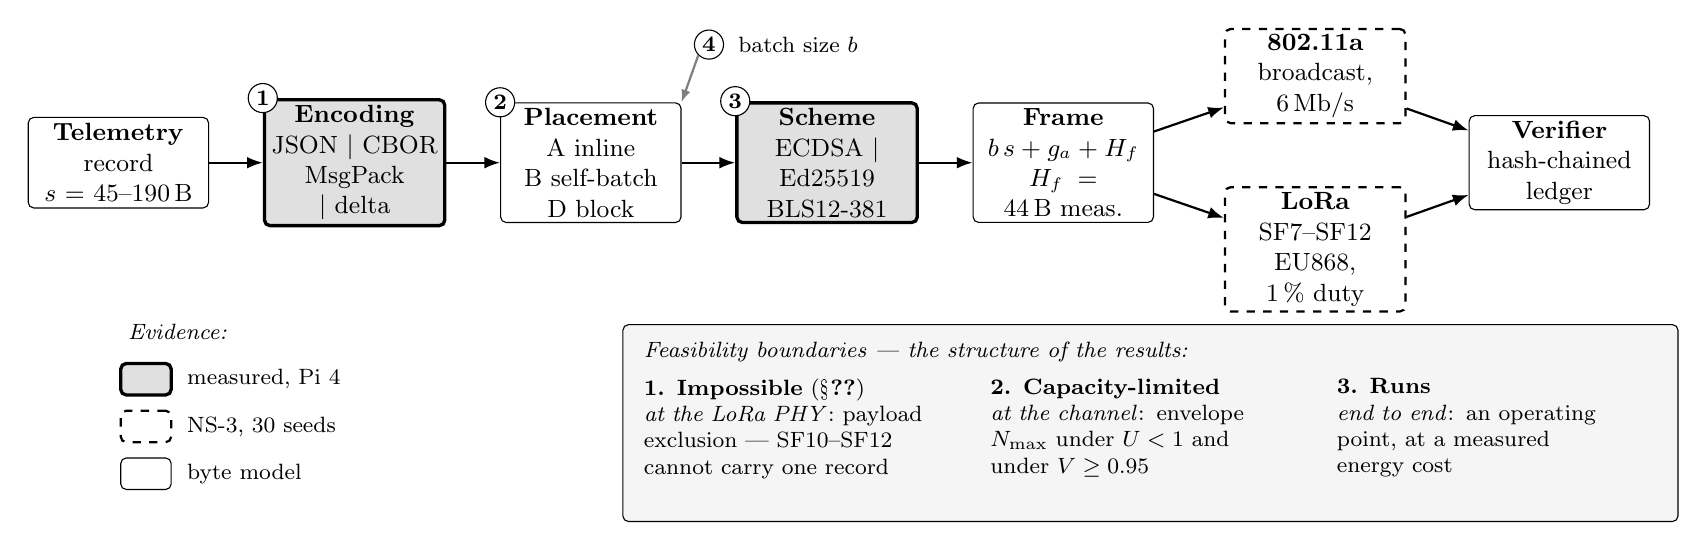
\begin{tikzpicture}[
  font=\small,
  blk/.style={draw, rounded corners=2pt, align=center, text width=2.15cm,
              minimum height=1.15cm, inner sep=2pt},
  meas/.style={blk, fill=black!12, very thick},
  sim/.style={blk, dashed, thick},
  mod/.style={blk},
  knob/.style={circle, draw, fill=white, font=\footnotesize\bfseries, inner sep=1.2pt},
  ar/.style={-{Latex[length=2mm]}, thick},
  bnd/.style={align=left, font=\footnotesize, text width=4.1cm},
  bar/.style={{Latex[length=1.6mm]}-, gray, thick, shorten <=1pt},
]

% ---- pipeline -------------------------------------------------------------
\node[mod]  (rec)   at (0,0)     {\textbf{Telemetry}\\ record\\ $s = 45$--$190$\,B};
\node[meas] (enc)   at (3.0,0)   {\textbf{Encoding}\\ JSON $\vert$ CBOR\\ MsgPack $\vert$ delta};
\node[mod]  (plc)   at (6.0,0)   {\textbf{Placement}\\ A inline\\ B self-batch\\ D block};
\node[meas] (sig)   at (9.0,0)   {\textbf{Scheme}\\ ECDSA $\vert$ Ed25519\\ BLS12-381};
\node[mod]  (frm)   at (12.0,0)  {\textbf{Frame}\\ $b\,s + \ba + H_f$\\ $H_f = 44$\,B meas.};
\node[sim]  (wifi)  at (15.2,1.1){\textbf{802.11a}\\ broadcast, 6\,Mb/s};
\node[sim]  (lora)  at (15.2,-1.1){\textbf{LoRa} SF7--SF12\\ EU868, 1\,\% duty};
\node[mod]  (led)   at (18.3,0)  {\textbf{Verifier}\\ hash-chained\\ ledger};

\foreach \a/\b in {rec/enc, enc/plc, plc/sig, sig/frm} \draw[ar] (\a) -- (\b);
\draw[ar] (frm) -- (wifi);
\draw[ar] (frm) -- (lora);
\draw[ar] (wifi) -- (led);
\draw[ar] (lora) -- (led);

% ---- the four design axes -------------------------------------------------
\node[knob] at (enc.north west) {1};
\node[knob] at (plc.north west) {2};
\node[knob] at (sig.north west) {3};
\node[knob] (k4) at (7.5,1.5) {4};
\node[font=\footnotesize, anchor=west] at (7.75,1.5) {batch size $b$};
\draw[gray, thick, {Latex[length=1.6mm]}-] (plc.north east) -- (k4.south west);

% ---- the three boundaries -------------------------------------------------
% No connector lines: all three boundaries bite at the right-hand end of the pipeline, so
% left-to-right arrows would cross. Each names its locus in words instead.
\node[draw, rounded corners=2pt, fill=black!4, anchor=north west,
      minimum width=13.4cm, minimum height=2.5cm] (band) at (6.4,-2.05) {};
\node[anchor=north west, font=\footnotesize\itshape] at (6.55,-2.15)
  {Feasibility boundaries --- the structure of the results:};
\node[bnd, anchor=north west] at (6.55,-2.62)
  {\textbf{1. Impossible} (\S\ref{sec:t6})\\ \emph{at the LoRa PHY}: payload\\
   exclusion --- SF10--SF12\\ cannot carry one record};
\node[bnd, anchor=north west] at (10.95,-2.62)
  {\textbf{2. Capacity-limited}\\ \emph{at the channel}: envelope\\
   $N_{\max}$ under $U<1$ and\\ under $V \geq 0.95$};
\node[bnd, anchor=north west] at (15.35,-2.62)
  {\textbf{3. Runs}\\ \emph{end to end}: an operating\\
   point, at a measured\\ energy cost};

% ---- provenance legend ----------------------------------------------------
\node[anchor=west, font=\footnotesize\itshape] at (0.0,-2.15) {Evidence:};
\node[meas, text width=0.5cm, minimum height=0.4cm] at (0.35,-2.75) {};
\node[anchor=west, font=\footnotesize] at (0.75,-2.75) {measured, Pi~4};
\node[sim, text width=0.5cm, minimum height=0.4cm] at (0.35,-3.35) {};
\node[anchor=west, font=\footnotesize] at (0.75,-3.35) {NS-3, 30 seeds};
\node[mod, text width=0.5cm, minimum height=0.4cm] at (0.35,-3.95) {};
\node[anchor=west, font=\footnotesize] at (0.75,-3.95) {byte model};

\end{tikzpicture}}
\caption{System model and the provenance of every stage. Four design axes
(\raisebox{0.2ex}{\textcircled{\scriptsize 1}}--\raisebox{0.2ex}{\textcircled{\scriptsize 4}}) are
searched jointly; only encoding and placement interact appreciably
(Table~\ref{tab:decomp}). Shading records \emph{what kind of evidence} supports each stage: shaded
blocks are measured on hardware, dashed blocks are simulated and validated against closed-form
models over 30 seeds, plain blocks are the byte model itself. The three boundaries below are the
paper's structure --- a configuration is impossible, capacity-limited, or it runs.}
\label{fig:system}
\end{figure*}


Fig.~\ref{fig:system} gives the pipeline, the four design axes, and
the kind of evidence behind each stage.

A record is integer-only fixed-point (floats break canonical-CBOR determinism) with a 32\,B
\texttt{prev\_hash} chain link; its encoded size is $s$. A frame carries $b$ records, a header $H_f = 44$\,B
\emph{measured} from the implemented wire format, and an authentication object $\ba$ (64\,B Ed25519/ECDSA, 96\,B BLS), bounded by the MTU
$M = 1500$\,B. On-air bytes per record, by placement:
\begin{align}
\text{A (inline)} &: s + \ba + H_f/b, \label{eq:A}\\
\text{B (self-batch)} &: s + (\ba + H_f)/b, \label{eq:B}\\
\text{D (block, $n$ frames)} &: s + (\ba + n H_f)/b. \label{eq:D}
\end{align}

\subsection{T1: overhead dominance}
For inline authentication the pure-authentication fraction is
\begin{equation}
\varphi = \frac{\ba}{s+\ba}.
\end{equation}
For $s = 45$--$190$\,B and $\ba=64$\,B, $\varphi = 25$--$59\%$: the smaller the payload, the more the
signature dominates. T2--T5 quantify what can be done about this, and where it stops.

\subsection{T2: batching cure and amplification}
Self-batch folds $b$ records under one signature, so the per-record auth cost $(\ba+H_f)/b \to 0$.
Packing to the MTU gives a goodput amplification over single-record framing:
\begin{equation}
A = \frac{M}{M - H_f - \ba},
\end{equation}
since at the MTU-filling batch $b_{\max}$ the frame $\approx M$ and $b_{\max}s \approx M-H_f-\ba$.
Inline (A) can \emph{never} amortize its per-record signature (only $H_f/b$ shrinks).

\textbf{T2a: when does $A$ apply?} (\emph{applied analysis, not a new result} --- the
diminishing-returns structure below is standard in the packet-aggregation literature.) The derivation assumes the \emph{MTU} caps the batch. Under a
freshness bound the cap is instead $b=\lfloor\Lambda D_{\max}\rfloor$, which does not depend on $s$;
then $C(s)=s+(\ba+H_f)/b$ and $dC/ds=1$ \emph{exactly}---compression pays $1\times$, not $A\times$,
and the residual authentication cost is a floor compression cannot reach. The boundary is
$s<(M-H_f-\ba)/(\lfloor\Lambda D_{\max}\rfloor+1)$. At $\Lambda{=}20$\,rec/s and
$D_{\max}{=}250$\,ms this is $232.0$\,B on 802.11, above every encoding studied, so
\textbf{$A$ is never operative there}; on a low-rate link ($M{=}222$) the MTU binds again and
$A{=}1.95$ \emph{is} operative. The ``compression pays $\times A$'' leverage is therefore real and
\emph{exclusive to low-rate links}.

\subsection{T3: loss-robustness frontier}
Let $p$ be per-frame loss and $V=\Pr[\text{a received record is independently verifiable}]$. Self-batch
frames self-verify, so $V_B = 1-p$, \emph{independent of $b$}. A block signature spanning
$n(b)=\lceil (bs+\ba+H_f)/M\rceil$ frames needs all fragments, so $V_D = (1-p)^n$. Whenever $n>1$,
$V_B = 1-p > V_D = (1-p)^n$: self-batch Pareto-dominates the marginal byte saving of over-aggregation.

\subsection{T4: power-independent scheme crossover}\label{sec:t4}
Per-record energy is $E = P_c\,(\text{CPU time}) + P_r\,(\text{radio time})$. Comparing Ed25519 and
BLS, which wins depends on the powers \emph{only} through their ratio $\kappa = P_r/P_c$:
\begin{equation}
\text{BLS wins} \iff \kappa > \kappa^\ast = \frac{\Delta \text{CPU}}{\Delta \text{RADIO}},
\end{equation}
where $\Delta\text{CPU}$ is BLS's extra CPU and $\Delta\text{RADIO}$ its radio-time saving. $\kappa^\ast$
is the break-even power ratio, obtained without measuring a single watt. Wi-Fi receive power sits below
CPU-active power, so plausible platforms have $\kappa \lesssim 0.5$.

\subsection{T5: co-design optimum}
Enumerate $(e,\sigma,\text{placement},b)$ and take the Pareto front over $\{$min bytes, min energy,
min staleness, max $V\}$ subject to MTU fit, $V \geq 1-\epsilon$, freshness $D(b)\leq D_{\max}$, and
verify-throughput $t_{\text{verify}}(b)\,\Lambda \leq 1$. The optimum is the smallest deterministic
encoding under self-batch at the largest \emph{freshness}-feasible batch --- not the largest
MTU-feasible one. Which ceiling binds is itself a result (T2a): at telemetry rates fill time
dominates $D(b)$, so $b \lesssim \Lambda D_{\max}$ and the MTU is never reached.

\subsection{The payload-exclusion bound (applied, not new)}\label{sec:t6}
T1--T5 ask what a saved byte buys. This bound asks the prior question --- whether a link admits
authenticated telemetry at all. The inequality is not ours: Gündo{\u{g}}an et
al.~\cite{gundogan2021firmware} compute exactly this residual for 802.15.4/NDN, and the
post-quantum literature reports NIST signatures as incompatible with 5G SIB1's 372\,B limit. We
restate it because it delimits our contribution, and because one composition of it appears not to
have been made explicit (below). A frame that is independently verifiable must carry the header, the
authentication object and at least one record, so a link of maximum payload $M$ is usable iff
\begin{equation}
s_{\max}(M) = M - H_f - \ba \;\geq\; s_{\min}.
\label{eq:t6}
\end{equation}
Fragmenting an oversized signature is no escape: by T3 a unit spanning $n$ frames verifies with
probability $(1-p)^n$, so $V\geq 1-\epsilon$ forces $n \leq \lfloor\ln(1-\epsilon)/\ln(1-p)\rfloor$,
which is at most $1$ whenever $\epsilon \leq p$ --- fragmentation is excluded outright. Equation~\eqref{eq:t6} is therefore evaluated at
$n{=}1$ and is an exclusion, not an inconvenience. Both ingredients are individually known --- the
residual above, and that a fragmented unit needs every fragment --- but the consequence is worth
stating: the \emph{sliced-signature} workaround proposed for constrained links is unavailable in
any regime where the verifiability target is no looser than the loss rate.

Three tiers follow, and each names a different escape route: $M < \ba$ (only a smaller signature
helps --- no header design, encoding, batching or chaining can), $\ba \leq M < H_f+\ba$ (only a
leaner header), and $H_f+\ba \leq M < H_f+\ba+s_{\min}$ (the sole regime an encoder can attack, and
where T2's amplification is operative). Section~\ref{sec:lowrate} applies this to LoRa.

\subsection{Channel and energy models}
At the 6\,Mb/s OFDM base rate, broadcast airtime is $T_{\text{air}}(L)=T_{\text{phy}}+8(L+\text{MAC})/R
+\text{DIFS}+\delta$ (fixed part $\approx 100${\us}); unicast adds SIFS and an ACK ($\approx 156${\us}).
Under contention among $N$ saturated stations, the Bianchi DCF fixed point is
\begin{align}
\tau = \frac{2(1-2p_c)}{(1-2p_c)(W+1)+p_c W\left(1-(2p_c)^m\right)}, \\
p_c = 1-(1-\tau)^{N-1}, \nonumber
\end{align}
with $W=16$, $m=6$, solved by damped iteration; saturation throughput $S = P_{tr}P_s\,8L/E[\text{slot}]$.
Self-batch per-record energy is $E = P_c(t_{\text{enc}}+2t_{\text{hash}}+t_{\text{sign}}/b+
t_{\text{verify}}/b) + P_r\,T_{\text{air}}(\text{frame})/b$. The hash term is the chain link
$\mathit{prev\_hash}=H(\text{record})$, charged twice per record because the sender extends the
chain and the receiver re-verifies it; unlike the signature it does \emph{not} amortize over $b$.

\section{Implementation and Validation}\label{sec:impl}
Everything reported here is produced by one codebase, from measured inputs, under a fixed
reproduction procedure. We describe what was built and how each component was checked, because the
credibility of a feasibility boundary rests entirely on the models that draw it.

\textbf{Encoders and schemes.} Four record encodings (JSON, CBOR, MessagePack, and a delta codec
with a keyframe every $K{=}16$ records) and three signature schemes (ECDSA-P256, Ed25519, BLS12-381)
are implemented behind one interface. Records are integer-only fixed point: floating point breaks
canonical-CBOR determinism, and a non-deterministic encoding cannot be hash-chained. Each scheme is
checked against published known-answer vectors (RFC~8032, Wycheproof, the Chia BLS suite) before any
timing is taken.

\textbf{Timing harness.} Crypto and encode timings are medians over repeated runs with the garbage
collector disabled, a warmup phase, a checksum on the work performed to prevent dead-code
elimination, and bootstrap confidence intervals. Timings used by the optimizer are measured
\emph{on the Raspberry~Pi~4 target}, not on the development host: the two disagree on which
signature scheme is faster (Sec.~\ref{sec:t4}), so using x86 numbers would select the wrong scheme.

\textbf{Wire format and placements.} A hash-chained store produces canonical-CBOR wire vectors, from
which the frame header is \emph{measured} at $H_f{=}44$\,B rather than assumed. All four placements
are implemented over that format, so the byte model is validated against bytes actually emitted.

\textbf{Channel model.} The 802.11a airtime model keeps broadcast and unicast separate --- they are
not the same model with an ACK removed, which Sec.~\ref{sec:results} shows quantitatively. Both are
validated against NS-3~3.48 over 30 seeds, and the broadcast airtime is additionally checked against
two Raspberry~Pi~4 radios.

\textbf{Optimizer.} An exhaustive search over (encoding $\times$ scheme $\times$ placement $\times$
batch) evaluates the byte, energy, freshness and verifiability models at every point and returns the
Pareto front, so the reported optimum is not the output of a heuristic.

\textbf{Reproduction procedure.} Every artifact carries an environment and configuration-hash
header. A gate re-derives all 16 model-derived artifacts byte-identically on each commit and fails
if any differs; artifacts requiring NS-3 or the hardware rig cannot be re-derived in that gate and
are labelled as such rather than counted as reproduced. Figures are regenerated from the same frozen
CSVs, and a separate check asserts that every figure the paper cites is still produced by a
generator that runs --- added after three figures were found plotting superseded constants
(Sec.~\ref{sec:repro}).

\section{Results}\label{sec:results}

\textbf{Three boundaries, in order of how durable they are.} The question an operator has is not
how many bytes a scheme saves but \emph{which configurations can run at all}. We answer it as three
separate boundaries, and we order them by how likely each is to survive contact with a better model:

\begin{enumerate}
\item \textbf{Impossible} (Sec.~\ref{sec:lowrate}). A link whose payload cannot hold one header, one
signature and one record admits no per-frame-verifiable telemetry at \emph{any} encoding, batch or
scheme. With a measured $H_f{=}44$\,B this excludes four of seven EU868 data rates. It is
arithmetic, so unlike everything else here it cannot move.
\item \textbf{Capacity-limited} (Table~\ref{tab:envelope}). Above that floor the binding constraint is the
shared medium. Coupling the byte model to an NS-3-validated broadcast model gives the largest
neighbourhood each configuration sustains: the co-design carries $1.9$--$3.2\times$ the inline
baseline, reported at two thresholds because they answer different questions.
\item \textbf{Runs} --- and what it costs. The byte reduction ($58.7\%$ total,
$72.0$\,B/record) is best read as the \emph{mechanism} that moves the boundary outward, not as the
result. Its authentication component reduces to $1-1/b$ and is invariant to header size, signature
size, encoding and scheme, so quoting it as a headline would credit four axes for what two produce.
\end{enumerate}

The airtime model underneath boundary~2 is validated twice: against NS-3 over 30 seeds, and against
two Raspberry~Pi~4 radios, where the predicted $1.988$\,ms broadcast airtime measures $1.995$\,ms,
a $0.36\%$ gap (equivalently, a $502.98$\,fps ceiling measured at $501.19$).

All values are from frozen CSVs. Byte and model results were derived on an x86 host
(Intel~i5-14400F); the crypto timings, encode timings and both power figures feeding the energy
column are \emph{measured on the Raspberry~Pi~4} thesis platform (decision D8), so the energy
column is platform-consistent ARM throughout.

\begin{table}[t]\centering\footnotesize
\caption{E1: overhead dominance (T1), 30 seeds. $\varphi = 64/(s+64)$.}
\label{tab:e1}
\begin{tabular}{lrr}
\toprule
encoding & mean bytes $s$ & $\varphi$ \\
\midrule
JSON & 191.1 & 25.1\% \\
CBOR & 66.25 & 49.1\% \\
MessagePack & 65.16 & 49.6\% \\
\textbf{delta} & \textbf{45.00} & \textbf{58.7\%} \\
\bottomrule
\end{tabular}
\end{table}

\textbf{E1 (Table~\ref{tab:e1}).} The auth fraction climbs from 25\% (JSON) to 59\% (delta): compressing
the payload makes a fixed 64\,B signature dominate---T1 confirmed.

\textbf{P1 crypto (x86 medians).} ECDSA-P256 sign/verify $26.2/78.5${\us}; Ed25519 $29.1/95.0${\us}; BLS
$324.6/1016.5${\us}; BLS aggregate-verify$(b{=}8)$ $3445${\us}. Notably, ECDSA \emph{beats} Ed25519 on
x86 (OpenSSL P-256 assembly)---the reverse of the usual ordering. The ordering \emph{flips} on the
ARM target (Ed25519 259.5 vs ECDSA 326.9{\us} verify), which is what the optimizer uses; both are
64\,B, so the byte results are identical either way. Because both are 64\,B the tie is broken on
measured energy, and on the ARM target that selects \textbf{Ed25519} --- which is what the
optimizer reports.

\textbf{E2 (T2/T2a).} At MTU 1500, self-batch, the measured amplification
$A_{@b}=(\text{bytes/rec})/s$ matches $A = M/(M-H_f-\ba)$ within $5\%$ (integer-$b$ slack, shrinking
with $s$); delta reaches $b_{\max}=30$ with $A_{@b}=A=1.0776$ exactly. The MTU sweep also straddles
the T2a boundary: $M{=}256$ is MTU-limited ($A{=}1.73$ realised), while $M{=}576$ and $M{=}1500$ are
freshness-limited and realise $A{=}1.0000$---i.e.\ the $b_{\max}{=}30$ above is \emph{unreachable}
at telemetry rates.

\textbf{E3 (T3).} $V_B \approx 1-p$ flat in $b$ (0.90 at $p{=}0.10$); $V_D=(1-p)^n$ drops the moment a
block spans $n>1$ frames (0.81 at $p{=}0.10$, $b{=}40$)---the frontier is exactly T3.

\textbf{E4 (T4, Fig.~\ref{fig:e4}).} On ARM---the thesis platform---Ed25519 verify is $33.2\times$
cheaper than BLS verify ($10.7\times$ on x86). Across the
full relay-fraction $\times$ batch $\times$ rate grid (80 points), Ed25519 wins \emph{every} one
(minimum $\kappa^\ast = 31.6 \gg 0.5$). At 96\,B, BLS carries more auth bytes than Ed25519 on own
self-batch traffic ($\kappa^\ast=\infty$) and saves bytes only on relay traffic for $b\geq 2$; its
$33.2\times$ verify cost on ARM keeps Ed25519 optimal for any plausible power ratio.

\begin{figure}[t]\centering
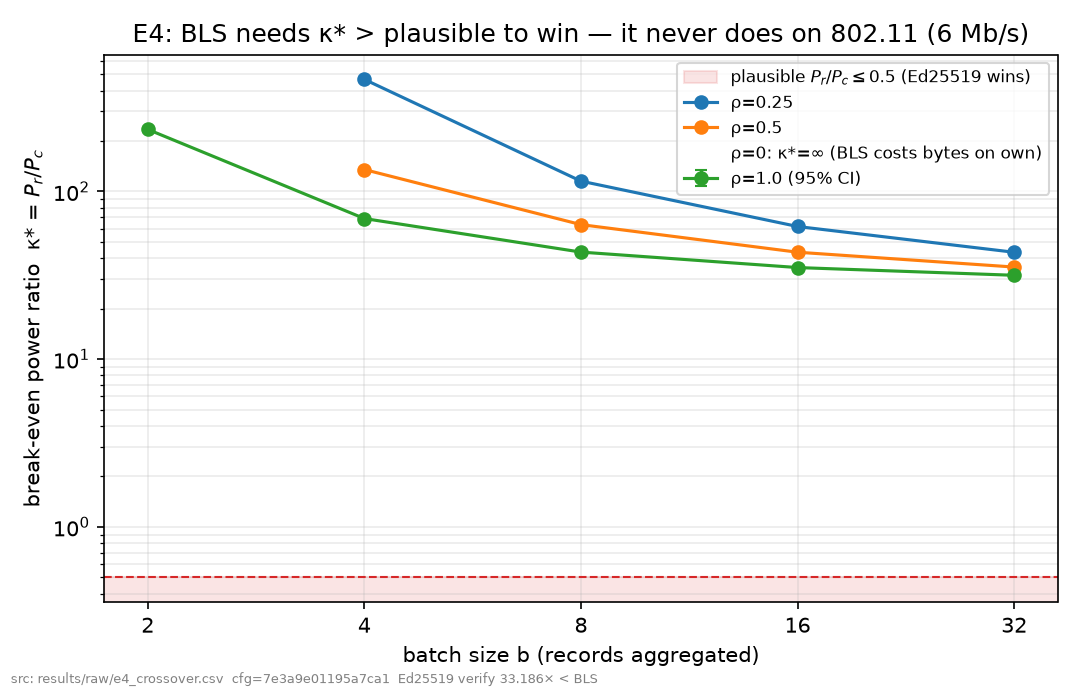
\includegraphics[width=\columnwidth]{e4_crossover.png}
\caption{E4: break-even power ratio $\kappa^\ast(b)$ per relay fraction. Every curve sits far above the
plausible band ($\kappa \leq 0.5$), so Ed25519 wins on 802.11; the $\rho{=}0$ curve is $\infty$ (BLS
costs bytes on own traffic).}
\label{fig:e4}
\end{figure}

\begin{table*}[t]\centering\footnotesize
\caption{E5: co-design headline (T5) under $V\geq0.95$, $p{=}0.05$ and $D\leq250$\,ms.
Total-byte cut $=(174.3-72.0)/174.3=58.7\%$; auth cut $=(108-27.0)/108=75.0\% \geq 40\% \Rightarrow$ PASS.
$H_f{=}44$\,B is measured from the implemented wire format, not assumed.}
\label{tab:e5}
\begin{tabular}{llll r r r r}
\toprule
config & enc & $\sigma$ & place & auth B/rec & total B/rec & $V$ & $D$ (ms) \\
\midrule
\textbf{optimized} & delta & Ed & B,$b{=}4$ & \textbf{27.00} & \textbf{72.00} & 0.95 & 200 \\
A+CBOR (Pillar-1) & cbor & Ed & A & 108.0 & 174.25 & 0.95 & 50 \\
A+JSON (naive) & json & Ed & A & 108.0 & 299.09 & 0.95 & 51 \\
D-over-agg & cbor & Ed & D,$b{=}40$ & 3.80 & 70.05 & 0.9025 & 2004 \\
\bottomrule
\end{tabular}
\end{table*}

\begin{table}[t]\centering\footnotesize
\caption{Attribution of the E5 saving. The authentication term is $1-1/b$ and is invariant to $H_f$,
$g_a$, encoding and scheme; the encoding term moves payload only. Reporting the single 75.0\% figure
would credit four axes for what two produce.}
\label{tab:decomp}
\begin{tabular}{l l r r}
\toprule
axis & what it moves & reduction & share \\
\midrule
placement $\times$ batching & auth B 108$\to$27.0 & 75.0\% & 79.2\% \\
encoding & payload B 66.25$\to$45.0 & 32.1\% & 20.8\% \\
scheme & neither (both 64\,B) & --- & --- \\
\midrule
\textbf{combined} & \textbf{total B 174.3$\to$72.0} & \textbf{58.7\%} & 100\% \\
\bottomrule
\end{tabular}
\end{table}

\begin{table}[t]\centering\footnotesize
\caption{Feasibility across the operating region, not at one chosen point (802.11a 6\,Mb/s,
broadcast model of~\cite{machen2007}). $N_{\max}$ is given at both thresholds: saturation ($U<1$)
and the measured $V{\geq}0.95$ boundary ($U{\approx}2.44$, interpolated between the
measured $U{=}2.23$ and $U{=}3.34$ rows). Batch obeys $b \leq \Lambda D_{\max}$,
so \textbf{bytes depend only on the product} --- the first two blocks are byte-identical and differ
only in capacity and in compliance.}
\label{tab:envelope}
\setlength{\tabcolsep}{4pt}
\begin{tabular}{l r r r r r r}
\toprule
configuration & $\Lambda$ & $D_{\max}$ & $b$ & \multicolumn{3}{c}{$N_{\max}$} \\
 & (rec/s) & (ms) & & $U{<}1$ & $V{\geq}0.95$ & $V{\geq}0.95$ \\
 & & & & & (mean) & (per run) \\
\midrule
\multicolumn{7}{l}{\emph{Primary: compliant with 3GPP TS~22.125}~\cite{3gpp_ts22125}} \\
\textbf{optimized} delta/B & 50 & 100 & 4 & \textbf{35} & \textbf{100} & 64--91 \\
A+CBOR (Pillar-1) & 50 & 100 & 1 & 18 & 31 & 24--29 \\
\midrule
\multicolumn{7}{l}{\emph{Relaxed freshness: same bytes, larger swarm, exceeds the standard}} \\
optimized delta/B & 20 & 250 & 4 & 103 & 213 & 163--201 \\
A+CBOR (Pillar-1) & 20 & 250 & 1 & 32 & 88 & 54--80 \\
A+JSON (naive) & 20 & 250 & 1 & 25 & 53 & 35--48 \\
\midrule
\multicolumn{7}{l}{\emph{Compliant but below the batching threshold} ($\Lambda D_{\max} < 4$)} \\
optimized delta/B & 20 & 100 & 1 & 34 & 98 & 62--89 \\
optimized delta/B & 10 & 100 & 1 & 78 & 180 & 134--169 \\
\bottomrule
\end{tabular}
\end{table}

\textbf{E5 (Table~\ref{tab:e5}, Fig.~\ref{fig:e5}).} The optimizer selects delta + Ed25519 +
self-batch at $b{=}4$, cutting total on-air bytes from 174.3 to \textbf{72.0\,B/record}---a
\textbf{58.7\%} reduction versus the Pillar-1 baseline at $V=0.95$, $p=0.05$. Hand-checked:
$45.0+108/4=72.0$\,B/record. The same $b{=}4$ is reached at either operating point, with freshness
$4/50=80$\,ms at the adopted compliant point and $4/20=200$\,ms at the relaxed one.

\textbf{Feasibility is the co-design result (Table~\ref{tab:envelope}).} The substantive claim is not
how many bytes are saved but which configurations \emph{can run}. Coupling the byte model to the
broadcast channel model gives the largest neighbourhood each configuration sustains. Two thresholds
are reported because they answer different questions. \emph{Saturation} throughput ($U<1$) is what
the medium carries when every node is backlogged, and it is conservative: simulation shows $98.9\%$
delivery still at $U{=}1$, with \emph{measured} verifiability $V_{\mathrm{meas}}$ crossing $0.95$
only near $U{\approx}2.44$. We
report both rather than choose, because choosing would select the flattering one.

A third column is reported because the second one is a statement about a \emph{mean}. The
$V{\geq}0.95$ crossing is located where the mean delivered fraction across seeds meets the target,
but $V$ is a reliability requirement, and at the crossing the distribution straddles it: at
$U{=}2.23$ the mean is $0.962$ while $10$ of $30$ seeds fall below $0.95$. Reading the criterion
per realisation instead---at least $95\%$ of runs must individually meet $V$---places the crossing
in $U \in (1.67, 2.23]$ and gives the ranges in the last column. We headline the mean, because it is
the reading under which the two thresholds are computed consistently, and report the per-run figures
beside it because they are what an operator promising a reliability target would need. \textbf{The
co-design advantage is insensitive to the choice}: the ratio spans $1.94\times$--$3.23\times$ under
the mean reading and $2.51\times$--$3.14\times$ under the per-run reading, so the conclusion does not
depend on which criterion a reader prefers.

Across the operating region the co-design multiplies the supportable swarm by between
$1.9\times$ and $3.2\times$ (Table~\ref{tab:envelope}): $1.94\times$ and $3.23\times$ at the two
thresholds for the compliant point, $3.22\times$ and $2.42\times$ for the relaxed one. \textbf{The
advantage is robust in existence and variable in size}, and we state it that way; a single
``${\approx}3\times$'' would be true of two of those four numbers and misleading about the other
two. What no single axis produces is the advantage itself: it needs the encoding (frame size) and the
placement--batch pair (frames per second) \emph{together with} the channel model. The scheme axis is
byte-neutral here and contributes nothing to this figure; it is decided on energy instead (T4).

\begin{figure}[t]\centering
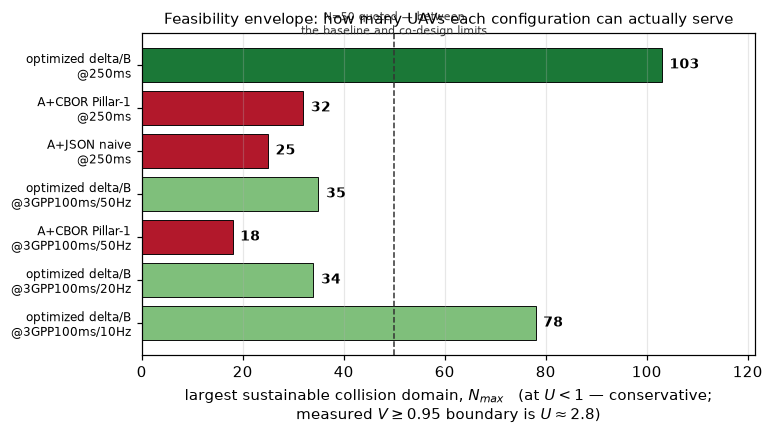
\includegraphics[width=\columnwidth]{fig_envelope.png}
\caption{Boundary~2. Largest single collision domain each configuration sustains. This is the
result that requires the coupling: the byte model alone cannot produce it, and the channel model
alone does not know the frame size. The co-design advantage is visible as horizontal displacement,
and it is variable in size --- see Table~\ref{tab:envelope} for both thresholds.}
\label{fig:envelope}
\end{figure}

\textbf{Choosing the operating point, and what it costs (item B3).} Because $b \leq \Lambda D_{\max}$,
\emph{only the product} $\Lambda D_{\max}$ sets the batch, and therefore the bytes. Two very
different operating points give the same $b{=}4$ and the same $72.0$\,B/record: $(20\,\text{Hz},
250\,\text{ms})$ and $(50\,\text{Hz}, 100\,\text{ms})$. They are not equivalent, because 3GPP
TS~22.125~\cite{3gpp_ts22125} requires ${\geq}10$\,msg/s \emph{and} ${\leq}100$\,ms latency, which
the first violates. \textbf{We adopt the compliant point $(50\,\text{Hz}, 100\,\text{ms})$ as
primary.} It is not a contrived rate: $50$\,Hz is PX4's \texttt{MAVLINK\_MODE\_ONBOARD} companion
stream rate, read from \texttt{mavlink\_main.cpp}~\cite{px4_mavlink_streams}; ArduPilot's
defaults are vehicle-specific rather than a single rate~\cite{ardupilot_stream_rates}. The byte result is unchanged; what it costs is
swarm size, $213 \to 100$ at the $V{\geq}0.95$ boundary and $103 \to 35$ at saturation. The relaxed
point is retained in Table~\ref{tab:envelope} because a deployment outside the standard's scope may
prefer it, and because reporting only the compliant point would hide the size of the trade.

The region also has a floor. Keeping $b \geq 4$ under a $100$\,ms bound needs $\Lambda \geq 40$\,Hz;
at $20$ or $10$\,Hz the same deadline forces $b{=}1$ and the co-design collapses to a $12.2\%$
saving. \textbf{The batching benefit is therefore not available at every compliant operating point}
--- it requires a telemetry rate high enough that four records accumulate within the deadline, which
is a constraint on the application, not on the cryptography.

\textbf{Attributing the saving (Table~\ref{tab:decomp}).} We separate the axes rather than report one
figure, because they are not equal contributors. Authentication overhead per record is
$(H_f+g_a)/b$; the record size does not appear, so the auth-byte reduction
$\bigl[(H_f{+}g_a)-(H_f{+}g_a)/b\bigr]/(H_f{+}g_a) = 1-1/b$ is invariant to header size, signature
size, encoding and scheme. We verified this by substitution over $H_f\in\{20,40,80,200\}$\,B
$\times\,g_a\in\{48,64,96\}$\,B: all twelve give 75.0000\%, and measuring $H_f$ at 44\,B rather than
the assumed 40\,B moved it not at all. Independently, the frozen E2 data gives the same auth overhead
to three decimals for all four encodings. The encoding axis is nonetheless load-bearing---it spans
$3\times$ on total bytes---but it acts on payload, contributing 20.8\% of the saving against
placement and batching's 79.2\%. The scheme axis is byte-neutral here (Ed25519 and ECDSA are both
64\,B) and is decided on energy and verification throughput instead (T4).

\textbf{The pre-registered criterion, and how much of it was actually at risk.} The success
criterion---cut on-air authentication bytes by ${\geq}40\%$ versus A+CBOR while holding
$V_{\mathrm{tgt}} \geq 0.95$ at $p{=}0.05$---was committed to version control in the project's
initial scaffold, two days before the result it judges existed; both commits are in the public
history, so the ordering is checkable rather than asserted. We report it as pre-registered even
though our own later analysis showed the authentication ratio to be a weak headline: moving the
goalposts after seeing the data would be the larger error.

Its two halves were not equally at risk, and we state that rather than let the word
``falsifiable'' do work it has not earned. For the frame-level placements
$V_{\mathrm{tgt}} = 1-p$ independently of encoding, batch and scheme, so with $p$ fixed at $0.05$
and $\epsilon = 0.05$ the verifiability half is satisfied \emph{exactly, by construction}---indeed
feasibility requires $p \leq \epsilon$ identically, since $1-p$ is the best verifiability any
placement attains. \textbf{The byte reduction carried the falsifiability on its own.} Measured
verifiability, written $V_{\mathrm{meas}}$ throughout, is a separate quantity obtained from
simulation and is not what this criterion tested.

\textbf{Sensitivity to $p$.} Fixing $p{=}0.05$ invites the question of how much rides on it, so we swept it. The answer is that nothing does, until everything does: for every $p \leq \epsilon$ the optimizer returns the \emph{same} configuration (delta, Ed25519, self-batch $b{=}4$, $72.0$\,B/record) from the same $44$ feasible points, and at $p{=}0.051$ the feasible set is \textbf{empty}. This is not a gradient but the cliff of T3: frame-level placements attain $V=1-p$ at best, so $p > \epsilon$ excludes every configuration rather than shifting the choice among them. The operating point is therefore insensitive to $p$ in the only sense available --- and the sensitivity that matters is not to the value of $p$ but to whether it exceeds the target.

\textbf{Ablation: which axes actually interact.} A decomposition attributes a total and is possible
even when the axes are independent, so it cannot establish the co-design claim on its own. We
therefore ran the full factorial on bytes/record. Every interaction involving \emph{encoding} is
\textbf{exactly zero}---$s$ enters $s+(H_f{+}g_a)/b$ additively, so it cannot interact---while
placement$\times$batching is $-24.0$\,B/rec, equal in magnitude to placement's own main effect. That
equality is the signature of a pure interaction, and the closed form says why: the placement benefit
is $g_a(1-1/b)$, which is \textbf{identically zero at $b{=}1$}. Placement A and B are byte-identical
on a single-record frame; batching is what gives placement anything to amortize.

\textbf{So the coupling is real but narrower than ``four coupled knobs'' suggests}, and we state it
that way: one genuine two-axis interaction (placement$\times$batching), one additive contributor
(encoding, $146$\,B/rec of the saving and the largest main effect), and one axis that does not move
bytes at the operating point (scheme). The intuition that a smaller payload ``increases the value
of batching'' holds only on the \emph{percentage} scale---the absolute saving is $81.0$\,B for JSON,
CBOR and delta alike---and two effects that are additive on an absolute scale always appear to
interact once expressed as ratios.

\textbf{Which constraint binds is itself the result.} Ignoring freshness, the byte-optimal batch is
$b{=}30$ at the MTU knee, cutting 96.7\%---but the oldest record in such a batch waits
\textbf{1.50\,s}, $6.0\times$ over $D_{\max}$. Because fill time dominates the delay, the admissible
batch obeys $b\lesssim\Lambda D_{\max}$ \emph{independent of encoding and scheme}, so freshness binds
long before the MTU does at telemetry rates. The co-design answer is therefore a frontier, not a
point: $b{=}1{\rightarrow}4$ trades $0/50/66.7/75\%$ auth-byte reduction against $50/100/150/200$\,ms
of staleness, with sharply diminishing returns. Over-aggregation (D) is byte-competitive (3.60\,B)
but \emph{fails} $V\geq0.95$ ($0.9025=(1-p)^2$)---a live demonstration of the T3 frontier---and misses
freshness by $8\times$.

\begin{figure}[t]\centering
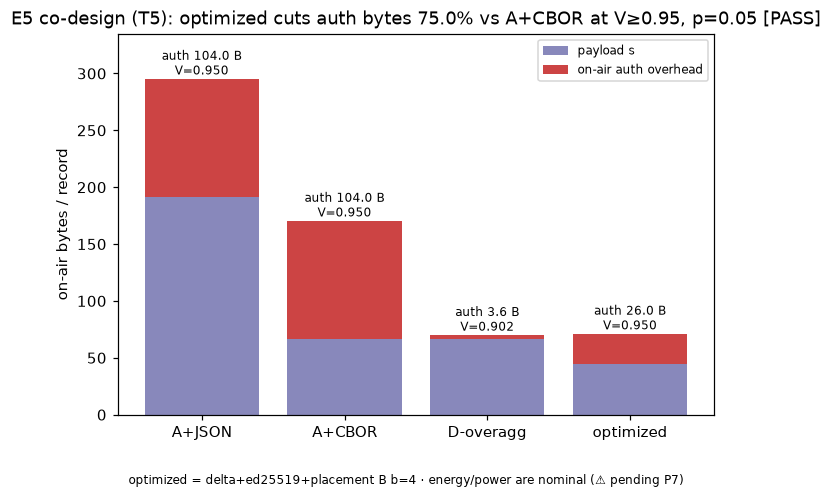
\includegraphics[width=\columnwidth]{fig_e5_codesign.png}
\caption{E5: on-air bytes/record (payload + authentication) for the optimized configuration versus the
baselines. Authentication overhead falls from $108$\,B to $27.0$\,B under the 250\,ms freshness bound
($H_f{=}44$\,B measured, $g_a{=}64$\,B, $b{=}4$).}
\label{fig:e5}
\end{figure}

\textbf{NS-3 validation (Table~\ref{tab:ns3}, Fig.~\ref{fig:ns3}).} Unicast validates the Bianchi
model~\cite{bianchi2000} to $+1.29$/$-0.40\%$ across $N=5$--$50$ (mean over 30 seeds; the
median-based derivation in Table~\ref{tab:ns3} gives $+1.33$/$-0.37\%$). Broadcast requires a \emph{different}
model, not the same one with the ACK removed. Reducing the unicast model by fixing $\tau=2/(W{+}1)$
under-predicts NS-3 by $17.3\times$ at $N{=}50$ (Table~\ref{tab:ns3}). PHY-trace instrumentation shows the cause is not frame
capture---which we measure at \textbf{0\%}, every successful decode arriving from a single-transmitter
busy period---but the \emph{backoff counter consecutive freeze process}: with no ACK the contention
window never doubles, so a station that has just transmitted may redraw a zero backoff and seize the
medium one slot ahead of every deferring station, whose counter is necessarily $\geq 1$. This is
precisely the effect analysed by Ma and Chen~\cite{machen2007,machen2008}, whose closed form reproduces
our measurements to within $0.51\%$ on throughput (30 seeds) and $2.49\%$ on the looser
success-probability and idle-slot-occupancy statistics; the
unicast counterpart is the ``anomalous slot'' analysis of Tinnirello \emph{et al.}~\cite{tinnirello2010},
which our unicast traces independently confirm. We claim no novelty for the mechanism; our contribution
is its validation at $W_0{=}16$ under 802.11a timing (the original studies used $W_0{=}32,128$ at
1\,Mb/s) and a direct slot-level measurement of it.

\begin{table}[t]\centering\footnotesize
\caption{Analytic DCF models vs.\ NS-3 3.48, relative gap $(\text{sim}-\text{model})/\text{model}$.
Median over 30 seeds, exact OFDM airtimes; regenerated from the frozen
\texttt{ns3\_contention.csv}. The naive reduction is the unicast model with $\tau$ fixed at
$2/(W{+}1)$, and it under-predicts by $17.3\times$ at $N{=}50$ --- the column exists to show
that broadcast needs a different model, not a modified one.}
\label{tab:ns3}
\begin{tabular}{rrrr}
\toprule
$N$ & unicast vs.~\cite{bianchi2000} & broadcast vs.~naive reduction & broadcast vs.~\cite{machen2008} \\
\midrule
5 & $+0.54\%$ & $+0.1\%$ & $-0.07\%$ \\
10 & $+1.33\%$ & $+3.4\%$ & $-0.12\%$ \\
20 & $+1.14\%$ & $+32.8\%$ & $+0.39\%$ \\
35 & $+0.24\%$ & $+268\%$ & $-0.56\%$ \\
50 & $\mathbf{-0.37\%}$ & $\mathbf{+1631\%}$ & $\mathbf{-0.27\%}$ \\
\bottomrule
\end{tabular}
\end{table}

\begin{figure}[t]\centering
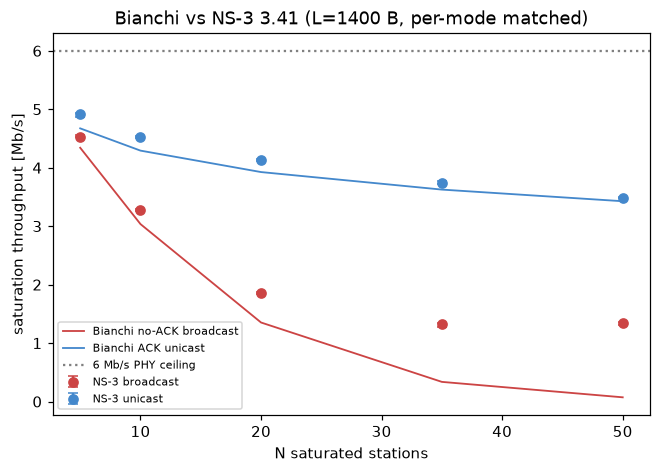
\includegraphics[width=\columnwidth]{fig_ns3_bianchi.png}
\caption{Analytic DCF models vs.\ NS-3 3.48 saturation throughput. Unicast matches Bianchi within
$+1.29$/$-0.40\%$ (mean, 30 seeds); broadcast matches Ma and Chen~\cite{machen2008} within
$0.51\%$, while the naive reduction of the unicast model (dashed) under-predicts by $17.3\times$ at $N{=}50$.}
\label{fig:ns3}
\end{figure}

\subsection{Comparison against a published external scheme}\label{sec:clas}
Every baseline so far is internal --- inline signing under different encodings --- which measures
improvement but not standing. The nearest published comparators are certificateless aggregate
signature (CLAS) schemes for vehicular broadcast, which target the same shape of problem: many
small, individually-attributable messages on a byte-constrained shared medium.

\textbf{A correction we had to make first.} Our byte model charged certificate bytes to \emph{no}
scheme, silently assuming out-of-band credential distribution. That assumption flatters public-key
infrastructure and penalises certificateless designs, whose entire advertised advantage is carrying
no certificate --- so comparing without it would have decided the result in our favour before any
measurement. We therefore charge certificates explicitly, using an ECDSA certificate of $162$\,B and
the transmission policy of the deployed standard, one full certificate every fifth
message~\cite{ndss2024pqv2v}.

\begin{table}[t]\centering\footnotesize
\caption{On-air cost per record against published CLAS schemes. CLAS figures are read from the
scheme's own comparison table under its own stated parameters~\cite{plos2025clas}; a $67$\,B traffic
message is subtracted to isolate security overhead.}
\label{tab:clas}
\begin{tabular}{lrr}
\toprule
 & total B/rec & security overhead \\
\midrule
Wang \emph{et al.} & 859 & 792 \\
Liang \emph{et al.} & 735 & 668 \\
Xu \emph{et al.} & 596 & 529 \\
Cahyadi \emph{et al.}~\cite{plos2025clas} & 583 & 516 \\
\midrule
AUTHBC, $b{=}4$, cert every 5th frame & \textbf{80.1} & 35.1 \\
AUTHBC, $b{=}4$, cert every frame & 112.5 & 67.5 \\
\bottomrule
\end{tabular}
\end{table}

\textbf{The informative result is not the ratio.} Every published CLAS overhead in
Table~\ref{tab:clas} is \emph{linear in the number of messages}: the aggregate compresses the
verifier's work, not the wire, because each message still carries its own identity, verification key
and signature components. Batching compresses the wire. \textbf{The two techniques operate on
different axes}, which is the same distinction we drew for receiver-side batch
verification~\cite{zhang2008batch}, now with a measurement rather than an argument.

\textbf{What this does not establish.} We do not claim to beat CLAS. Those schemes buy
\emph{conditional privacy} --- a per-message pseudonymous identity that an authority can trace ---
which AUTHBC does not provide and a provenance ledger arguably does not want. Part of their overhead
purchases a property we decline. Their group element is also $128$\,B against our $64$\,B signature,
so some of the gap is curve and encoding choice rather than design. The defensible statement is
narrower and more useful than a ratio: \emph{on a byte-constrained broadcast link, aggregate
signatures do not reduce airtime; placement and batching do.}

\section{Boundary 1 --- Impossibility: the Low-Rate Regime}\label{sec:lowrate}
Everything so far concerns a companion-class 802.11 link. The natural question is how far the
co-design carries, and the honest answer is that it stops --- which is not a caveat but the most
durable result in this paper. A capacity figure moves when the model improves; an exclusion does
not.

This section is \emph{analysis and simulation, not measurement}. No LoRa hardware was instrumented
and no LoRa energy figure is reported: the only metered radio power in this work is a Wi-Fi figure,
and reusing it would be fabrication. Every LoRa constant is transcribed from the SX1276 datasheet
(Rev.~7, \S4.1.1.5/\S4.1.1.7)~\cite{semtech_sx1276} and LoRaWAN RP002-1.0.3~\cite{lora_rp002}
(Tables~8 and~13, EU868 duty cycle $<1\%$).

\subsection{T6 excludes the four longest-range modes}
With $H_f = 44$\,B and a 64\,B Ed25519 signature, Eq.~\eqref{eq:t6} partitions EU868
(Table~\ref{tab:t6}). DR0--DR2 fail on the \emph{signature alone}: 64\,B does not fit a 51\,B
payload, so the exclusion holds even with a zero-byte header and a zero-byte record. The only
escape is a smaller authentication object, and the smallest standardised one is a 48\,B compressed
BLS12-381 $\mathbb{G}_1$ point~\cite{cfrg_bls} at 126-bit security --- which does fit 51\,B, leaving
three bytes for the header and the record together. DR3 fails on the encoding, and by six bytes. The $s_{\min}{=}13$\,B it is measured against is the smallest record this design can emit: the $45$\,B delta record of Table~\ref{tab:e1} minus the $32$\,B chain link, once chaining moves to once-per-frame (Sec.~\ref{sec:chaining}). That is the most favourable value available to us, so DR3's exclusion does not rest on a pessimistic choice --- a leaner record would have to beat $13$\,B while remaining hash-chainable.

\begin{figure}[t]\centering
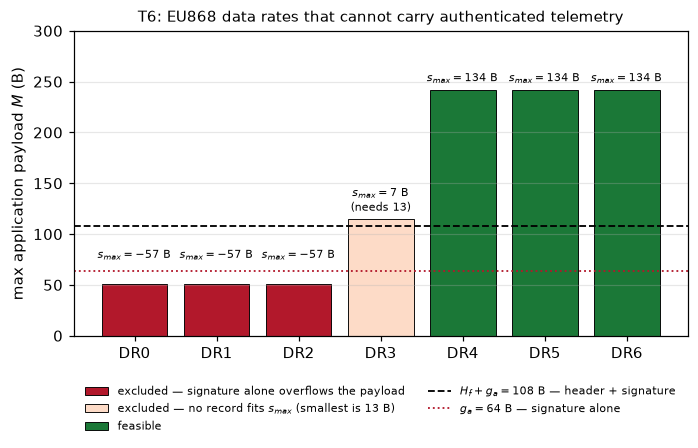
\includegraphics[width=\columnwidth]{fig_t6_exclusion.png}
\caption{Boundary~1. The payload-exclusion tiers across EU868 data rates at $H_f{=}44$\,B measured
and $g_a{=}64$\,B. DR0--2 are excluded by the signature alone --- no header design, encoding,
batching or chaining reaches them --- and DR3 misses on the record by six bytes. Only DR4--6 admit
per-frame-verifiable telemetry. The boundary is arithmetic, so unlike the capacity results it does
not move with the channel model.}
\label{fig:t6}
\end{figure}

\begin{table}[t]\centering\footnotesize
\caption{T6 applied to EU868 ($H_f{=}44$\,B measured, $\ba{=}64$\,B, $s_{\min}{=}13$\,B).}
\label{tab:t6}
\begin{tabular}{l r r l}
\toprule
DR & $M$ (B) & $s_{\max}$ & verdict \\
\midrule
0, 1, 2 & 51 & $-57$ & excluded --- signature alone overflows \\
3 & 115 & 7 & excluded --- no record fits (misses by 6\,B) \\
4, 5, 6 & 242 & 134 & feasible \\
\bottomrule
\end{tabular}
\end{table}

\subsection{Where the design changes: chaining}\label{sec:chaining}
On 802.11 freshness binds, so the batch is fixed by $\Lambda D_{\max}$ and saving payload bytes buys
nothing extra. On LoRa the \emph{regional payload limit} binds, so bytes convert directly into more
records per frame. Moving the 32\,B chain link from per-record to once-per-frame --- the receiver
re-derives the rest from $\mathit{prev\_hash}_{i+1}=H(\text{record}_i)$, leaving the stored ledger
byte-identical --- raises the DR5 batch from 2 to 7 and the sustainable rate from 0.060 to
$0.182$\,rec/s, a factor of $3.03$. We adopt it \emph{on this arm only}: the same change on 802.11
buys ${\approx}6\%$ energy and no extra records, which does not pay for losing independently
transmitted per-record tamper evidence.

\subsection{Capacity: the two penalties compound}
Time on air and the duty cycle are deterministic, so simulating them would be circular. One
quantity is not derivable that way --- how many nodes share the channel --- because LoRaWAN uplinks
are pure ALOHA, with no carrier sense and no acknowledgement. Simulating LoRaWAN scalability in ns-3
is established practice~\cite{vandenabeele2017scalability}, including proposals to replace the ALOHA
MAC with carrier sense~\cite{to2018loracsma} and recent extensions to non-terrestrial
links~\cite{traspadini2025lorantn}.

\textbf{A topology caveat, stated because it differs from the 802.11 arm.} LoRaWAN is by
specification a star-of-stars with no peer-to-peer mode: a recent FANET survey notes that it
``presents some limitations regarding its star topology, its medium access control (MAC) layer and
its lack of routing procedures''~\cite{paredes2023lorafanet}, and published peer-to-peer LoRa meshes
are built by discarding the LoRaWAN MAC entirely, ``not relying on LoRaWAN\ldots without the use of
gateways''~\cite{berto2021loramesh}. A LoRa FANET that was actually flown reports the same
constraint --- ``LoRaWAN only supports star topology'' --- and hybrid LoRa/802.11s UAV meshes
reach for a second radio for the same reason~\cite{davoli2021hybridlora}; having built one, it converges on a
\emph{single channel} and on dedicated transmit and receive radios to work around
half-duplex~\cite{zirak2021swarm}, which is the configuration we model. Nor is the gateway framing
unrepresentative of the multi-hop literature: a review of mesh proposals for LoRa finds that even
those pursuing flexible topologies retain ``a predominant nodes $\rightarrow$ gateway/sink data
flow'', with ``fewer proposals'' targeting genuinely decentralized architectures, and lists
``network scalability with hundreds, or even thousands, of nodes'' among the challenges that remain
open~\cite{centelles2021beyondstar}; concrete multi-hop LoRa deployments keep the same
sink-directed shape~\cite{abrardo2019multihoplora,jiang2020hybridlpwan}, and a 2025 ns-3 LoRa mesh
study states plainly that ``there is currently no standardised and commercialised multi-hop
LoRa-based network''~\cite{durand2025loramesh}. Our scenario is therefore $N$ end devices reporting to one
gateway, whereas the 802.11 arm is a genuine broadcast among peers. \textbf{The two arms bracket the
design space rather than repeating one experiment at two data rates}, and the low-rate result should
be read as the infrastructure-collected variant. What transfers
is the part that matters: collision statistics at a receiver depend on how many transmitters are
concurrently in range, not on what the receiver is attached to, so the measurement models a single
receiver in an ad hoc network with $N{+}1$ nodes. It is also why the single-demodulator provisioning
is the right one here and not, as it would be for a gateway, an artificially harsh one: \emph{a UAV
peer has one radio}. Two ad hoc effects remain outside the model. A half-duplex radio cannot receive
during its own $364$\,ms frame, costing a peer ${\approx}2\%$ of every other peer's frames, a loss no
gateway suffers --- and not an artifact of our setup, since Class A devices are specified as
half-duplex pure-ALOHA transceivers~\cite{paredes2023lorafanet} and peer-to-peer LoRa implementations
report designing around exactly this constraint~\cite{berto2021loramesh}. And $V$ is a \emph{per-receiver} metric, as in the 802.11 arm: a record reaching
\emph{every} peer in a single broadcast has probability ${\approx}(1-p)^{N-1}$, so single-hop full
replication is not what $V$ measures and would require gossip or relay --- an application-layer
mechanism we do not study. Simulating the AUTHBC frame at DR5
under the same $0.95$ threshold used for 802.11 --- here applied to \emph{measured} delivery
$V_{\mathrm{meas}}$, not to the assumed $V_{\mathrm{tgt}}$ of the byte model --- gives
$N_{\max} = 3$, with a sharp cliff: delivery is $0.960$ at $N{=}3$ and $0.917$ at $N{=}5$.
There is no backoff to absorb contention. We give this figure with its uncertainty, as we do on
the 802.11 arm: bootstrapping the crossing over the 30 seeds puts it at $3$ with a $95\%$ interval
of $[2,3]$, and at the certified $N{=}3$ the mean clears $0.95$ while \emph{nine of thirty}
individual runs do not. Read per realisation the value is $1$. The mean-based figure is the one
quoted, for consistency with the 802.11 thresholds, but a deployment promising a reliability target
should use the per-run reading.

This figure is far below the node counts usually quoted for LoRaWAN, and the discrepancy is
configuration, not disagreement. We simulate the LoRa physical layer --- real modulation, with the
module's measured interference and capture model --- but on its harshest MAC provisioning: a single
logical channel, a single gateway demodulation path, and one forced spreading factor, since the data
rate is a design variable here and each run therefore fixes it. Comparison with measurement-based
published results~\cite{bor2017lora} must respect that. Both studies transmit at the $1\%$
duty-cycle ceiling, so per-node occupancy is $1\%$ in both and offered load scales identically as
$G = 0.01N$; mapping their multi-channel result through their own fit
$f_{\mathrm{MCH,MSF}}(x) = f_{\mathrm{SCH,SSF}}(x/18)$ places their ${\approx}32\%$ loss at $56$
nodes on one channel and one SF, where we measure ${\approx}62\%$ at $N{=}50$. \textbf{Our model is
therefore roughly $2\times$ more pessimistic than theirs, not more optimistic}, most plausibly
because a single demodulation path rejects a second concurrent arrival outright instead of granting
it the capture chance their measurements support. Our own configuration is deliberately the pessimistic one in a further respect: the interference
matrix treats \emph{any} same-spreading-factor overlap as fatal, so there is no capture at all,
where a real LoRa receiver recovers the stronger of two colliding frames. Enabling a 6\,dB capture
threshold raises delivery by $2.7$ points at $N{=}8$ and by $1.29\times$ at $N{=}50$ without moving
$N_{\max}$. The small margin over the Poisson curve $e^{-2G}$ at low load is not capture but traffic
regularity: sources are periodic rather than Poisson, for which the escape probability is
$(1-2\tau/T)^{N-1} = 0.868$ at $N{=}8$ against $0.871$ measured.

\textbf{The result is also range-limited, and that limit binds before capacity does.} Our channel
model attributes all loss to collisions, and this is not an option we simply left switched off:
enabling correlated shadowing changes the outcome on no row at either $500$ or $1000$\,m. That is a
property of the link budget, not a wiring error --- with $14$\,dBm transmit power and the
$-130$\,dBm SF7 gateway sensitivity, log-distance path loss leaves $28.8$\,dB of margin at
$500$\,m and $17.5$\,dB at $1000$\,m, which an ${\approx}8$\,dB shadowing standard deviation cannot
erode; simulated failure onset is near $4200$\,m, and shadowing does bite there ($1.000$ falls to
$0.515$ at $4000$\,m). \emph{Our propagation parameters describe a considerably better link than a
real drone-to-drone channel, and no option the scenario exposes closes that gap.} Field measurements of
air-to-air LoRa on real drones~\cite{zirak2021swarm} show a link losing frames to range alone: PDR
falls from $0.9711$ at $200$\,m to $0.9550$ at $500$\,m and $0.9045$ at $1000$\,m, measured with
two drones and a base station, where contention is negligible. Since the two loss mechanisms are
independent, delivery is $P_{\text{link}}(d) \times P_{\text{no-coll}}(N)$, and any range whose link
PDR already misses the target makes it unreachable at \emph{every} node count. Composing their
measured link with our measured collision curve is sharper than either term alone:

\begin{center}\footnotesize
\begin{tabular}{lrrr}
\toprule
$V$ target & $200$\,m & $500$\,m & $1000$\,m \\
\midrule
$0.95$ & 1 & 1 & 0 \\
$0.90$ & 3 & 3 & 1 \\
$0.85$ & 5 & 5 & 3 \\
$0.80$ & 10 & 8 & 5 \\
\bottomrule
\end{tabular}
\end{center}

\textbf{At $V \geq 0.95$ the regime admits no multi-node network at all.} The link alone delivers
$0.9711$ at $200$\,m, leaving $0.0039$ of headroom, while our least-loaded measured point ($N{=}2$)
already spends $0.0283$ on collisions. A lone transmitter passes; two do not. The capacity figure is
therefore conditional not only on range but on the threshold: relaxing to $V \geq 0.90$ restores
$N_{\max} = 3$, and to $0.85$ restores $5$. We report the curve rather than a point because the
choice of threshold, not the physics, is what decides whether this regime is usable --- and that
choice belongs to the deployment, not to us. At the $1000$\,m radius our own scenario configures,
an idealised channel is $9.6$ percentage points optimistic; this mirrors the 802.11 arm, where the
idealised model is $39\%$ optimistic at $500$\,m.

\textbf{$N_{\max}=3$ should therefore be read as a worst-case bound at short range --- one channel,
one demodulator, one spreading factor, $d \leq 500$\,m --- rather than as a LoRaWAN network
capacity.} \textbf{It also carries wide uncertainty.} Every device transmits on one exact period and
ALOHA has no backoff, so relative phases are fixed for a whole run: a pair that collides once
collides always. Delivery is consequently bimodal rather than noisy about a mean --- over 30 seeds at
$N{=}5$, $22$ runs deliver exactly $1.000$ and the rest fall to $0.20$--$0.84$, giving a mean of
$0.891$ with $\sigma = 0.21$. A three-seed mean, which is what the figure above rests on, cannot
characterise that distribution. At realistic $\pm20$\,ppm crystal tolerance the accumulated drift
over an hour ($144$\,ms) is too small to break a $728$\,ms collision window, so the effect is
physical for a naive periodic sender; real LoRaWAN Class~A devices randomise transmission timing
precisely to avoid it, which the simulated sender does not model. We note that this
distribution is invisible in a literature that does not report replication: of the four ns-3 LoRa
simulation studies meeting our pre-registered inclusion criteria---including the foundational
scalability analysis~\cite{vandenabeele2017scalability}---none states a seed count, a confidence
interval or a standard deviation. The phenomenon itself is \emph{not} unobserved: Durand and
Booysen attribute their own bimodal delivery to nodes that ``always transmit on a specific SF, time,
and channel'', producing ``certain packet collisions being repeated for every transmission
cycle''~\cite{durand2025loramesh}. What is absent is any quantification of the resulting dispersion,
or the replication information a reader would need to detect it. We report the figure with this
caveat rather than restate it as a precise capacity. It is conservative
in the direction that matters least for the claim being made: the point of this section is that the
low-rate regime is qualitatively different, and a conservative bound does not manufacture that
difference, it understates the margin. It is conservative in one further respect: LoRaWAN Class~A
specifies pure ALOHA~\cite{paredes2023lorafanet} and we model it, whereas a purpose-built LoRa FANET
adds listen-before-talk~\cite{zirak2021swarm} and would collide less.

\subsection{What infrastructure collection would buy}\label{sec:lora-gateway}
The single-demodulator, single-channel provisioning above models a UAV peer. The complementary
question --- what if a ground gateway collected the ledger instead? --- is a configuration change,
and we ran it: three channels and eight demodulation paths, the RP002 provisioning, with the same
forced data rate. Delivery improves substantially and the improvement grows with load, reaching
$1.90\times$ at $N{=}50$ ($0.3755 \rightarrow 0.7134$) and still $0.5071$ at $N{=}100$, which the
peer configuration cannot reach at all. \textbf{Yet $N_{\max}$ moves only from 3 to 8} (95\% CI $[5,8]$; the bare value must not be quoted). The
$V \geq 0.95$ criterion sits on a near-vertical part of the delivery curve --- the gateway passes at
$N{=}8$ with $0.9526$ and fails at $N{=}10$ with $0.9398$ --- so a threefold reduction in offered
load per channel shifts the threshold barely at all. This is the same duality the 802.11 arm shows
between saturation and the measured verifiability boundary: \emph{a capacity metric and a
strict-reliability metric respond very differently to the same change}, and reporting either alone
would mislead.

\subsection{An external check on the low-rate capacity}\label{sec:lora-external}
The 802.11 arm is validated against two published analytical models. The low-rate arm rested on a
single simulator, so we gave it the same treatment. Bor \emph{et al.}~\cite{bor2017lora} publish
their capacity result in closed form --- a quintic fitted at $R^2 = 0.997$ to \emph{total} packet
loss (collisions plus wrong-payload-CRC) measured on SX1301 hardware --- which means it can be
\emph{evaluated at our operating point} rather than quoted at theirs. We implemented it, validated
the implementation against the four loss figures their own text states (three land within
${\approx}3$ points; the fourth is stated as collisions-only, so our total correctly exceeds it),
and applied the identical $V \geq 0.95$ criterion.

\begin{table}[t]\centering\footnotesize
\caption{The low-rate capacity, by two independent methods.}
\label{tab:lora-external}
\begin{tabular}{lrrl}
\toprule
$N$ & AUTHBC (NS-3) & Bor \emph{et al.} & \\
\midrule
2  & $2.8\%$ & $3.1\%$ & we are more optimistic \\
3  & $4.0\%$ & $3.8\%$ & crossover \\
5  & $8.3\%$ & $5.1\%$ & we are $1.64\times$ more pessimistic \\
8  & $12.9\%$ & $7.0\%$ & we are $1.85\times$ more pessimistic \\
30 & $43.0\%$ & $19.9\%$ & we are $2.16\times$ more pessimistic \\
50 & $62.5\%$ & $29.9\%$ & we are $2.09\times$ more pessimistic \\
\midrule
\multicolumn{2}{l}{$\mathbf{N_{\max}}$ \textbf{at} $\mathbf{V \geq 0.95}$} & & \\
& \textbf{3} & \textbf{4} & \\
\bottomrule
\end{tabular}
\end{table}

A discrete-event simulation of the LoRa physical layer and a polynomial fitted to hardware
interference measurements land \textbf{one node apart} on the quantity this section rests on
(Table~\ref{tab:lora-external}). The agreement should not be over-read --- below $N \approx 10$
their fit is dominated by a $1.78\%$ intercept that is an artifact rather than a measurement --- but
it is obtained independently and it is the right order. The disagreement in \emph{shape} is the more
informative part, and it matches the configuration difference: our runs model no capture at all and
a single demodulation path, where their measurement-based model grants both, so beyond the crossover at
$N{\approx}3$ we reject concurrent arrivals that their gateway would still recover.

\begin{table}[t]\centering\footnotesize
\caption{The low-rate regime is not a slower version of the same problem.}
\label{tab:lowrate}
\begin{tabular}{l r r r}
\toprule
 & per node & $N_{\max}$ & aggregate \\
\midrule
802.11a, delta/B, $b{=}4$ & 20 rec/s & 103 & 2060 rec/s \\
LoRa EU868 DR5, $b{=}6$ & 0.165 rec/s & 3 & 0.495 rec/s \\
\midrule
ratio & $121\times$ & $34\times$ & $\mathbf{\approx}\mathbf{4200}\boldsymbol{\times}$ \\
\bottomrule
\end{tabular}
\end{table}

The arm is ${\approx}120\times$ slower per node \emph{and} ${\approx}34\times$ smaller per domain,
and it is the product that matters (Table~\ref{tab:lowrate}). LoRa is not a slow 802.11; it is a
different regime, in which authenticated per-record telemetry is not the right application at all.
Its defensible role is long-range \emph{provenance} --- a tamper-evident trickle --- not live
telemetry.

One caveat of provenance. The simulator enforces RP002 Table~12 (repeater-compatible, 222\,B) while
our analytical model uses Table~13 (non-repeater, 242\,B); at DR5 that caps the batch at 6 rather
than 7. Both are defensible readings of the same standard, and we simulate what the implementation
accepts rather than reconcile them silently.

\section{Reproducibility and Scientific Integrity}\label{sec:repro}

\textbf{A simulator artifact large enough to change what a reader should believe.} The ns-3 LoRaWAN
module's periodic sender fires on an exact interval, and LoRaWAN ALOHA has no backoff, so relative
transmission phases are frozen for an entire run: a pair that collides once collides on every cycle.
Delivery becomes \emph{bimodal} rather than noisy about a mean. Over 30 seeds at $N{=}5$, 22 runs
deliver exactly $1.000$ and the rest fall to $0.20$--$0.84$. We measure the consequence: the
coefficient of variation is inflated \textbf{2--8$\times$} relative to a sender with one-second
transmission jitter, the inflation growing with node count ($2.9\times$ at $N{=}5$, $7.9\times$ at
$N{=}100$). Real LoRaWAN Class~A devices are required to randomise transmission timing; the module
does not.

\textbf{We claim the measurement, not the observation.} Durand and Booysen report the same effect
in their own results, attributing bimodal delivery to nodes that ``always transmit on a specific SF,
time, and channel'', producing ``certain packet collisions being repeated for every transmission
cycle''~\cite{durand2025loramesh}. What appears to be absent from the literature is any
\emph{quantification} of the resulting dispersion, and---of the four ns-3 LoRa simulation studies
meeting our pre-registered inclusion criteria---any statement of seed count, confidence interval or
standard deviation that would let a reader detect it. That is why every capacity figure in this
paper is reported at 30 seeds with its distribution, and why a threshold crossing is given as an
interval: at $N{=}3$ the mean clears $V{\geq}0.95$ while nine of thirty individual runs do not.

The survey protocol was committed to version control \emph{before} the corpus was assembled, and the
sweep is reproducible (\texttt{make survey-direction-c}). Papers whose text will not extract are
excluded from the denominator rather than scored as reporting nothing: one held PDF yields five
characters, and counting it as evidence would manufacture support for our own hypothesis.

Beyond the results, the project's second product is its discipline. Anomalies were root-caused, not
patched over: a stateful delta codec used statelessly (60$\to$45\,B); string-keyed CBOR replaced by
canonical arrays (110$\to$66\,B); the BLS size corrected 48$\to$96\,B (with the T4 model updated); and,
on the broadcast channel, three successive explanations retracted in writing---an ``18$\times$
capture'' over-claim, then the capture effect itself (PHY instrumentation measured it at 0\%), and
finally our own claim to have discovered the responsible mechanism, which a literature check showed had
been published in 2007~\cite{machen2007}. A whole-repo audit re-derived every formula against the code and hand-checked one point per
experiment. Finally, freezing raw data risks \emph{silent staleness}, so an automated gate re-derives
every deterministic frozen artifact from the current code and fails on any drift---verified to catch the
exact regression it was built for. No result is fabricated, no test skipped, no tolerance widened.

\section{Limitations and Future Work}

\textbf{Post-quantum signatures: a projection, not a contribution.} Practical PQ authentication for
vehicular broadcast is already solved at NDSS level~\cite{ndss2024pqv2v} and for 5G
broadcast~\cite{arxiv2510pqsib1}; we claim nothing there. But the substitution is mechanical in our
model, so we report it rather than leave a foreseeable question unanswered. Taking sizes from those
sources---ML-DSA/Dilithium2 at 2420\,B and SPHINCS+ at 7856\,B per signature---and holding the
adopted operating point, bytes/record at $b{=}4$ move from $72.0$\,B (Ed25519) to $661.0$\,B
($9.2\times$) and $2020.0$\,B ($28.1\times$).

\textbf{The binding problem is not the ratio, it is that batching cannot rescue it.} Two of our own
constraints collide. Freshness caps the batch at $b \leq \lfloor \Lambda D_{\max} \rfloor = 5$, so
there is almost nothing to amortize a kilobyte-scale signature over: reaching Ed25519's $27$\,B/record
of overhead would need $b{=}91$ for ML-DSA, a $1.83$\,s fill---$18\times$ the $100$\,ms deadline. And
the MTU binds harder still: an ML-DSA signature plus the $44$\,B header is $2464$\,B, which
\emph{exceeds the 1500\,B MTU on its own}, so placement B stops fitting in a single frame at
\emph{any} batch size. That is precisely why~\cite{ndss2024pqv2v} needs a fragmentation design
($\beta{=}4$ frames for Dilithium, $8$ for SPHINCS+ in their Table~III) rather than a larger batch.
Fragmenting authenticated payloads is itself a security surface in constrained
networks~\cite{sobati2025fragmentsec}, so the change is not only a byte-accounting one. PQ
identity-based signatures with aggregation are being proposed for fog-enabled FANETs
specifically~\cite{almajmaie2026pqfanet}; that line optimises signing and verification cost, which
is complementary to the wire-byte constraint that binds here.
The honest conclusion is that AUTHBC's amortization argument does not survive the transition
unchanged: a PQ variant would be a different design, not a re-parameterisation, and the placement
axis would have to be re-derived against fragmentation rather than against the MTU.

The 802.11 and LoRa arms are evaluated separately and are not combined into a single heterogeneous scenario; a gateway-relayed hybrid is future work. Energy is now measured on a Raspberry~Pi~4 with
INA219 meters ($P_\mathrm{cpu}=0.634$\,W, $P_\mathrm{radio}=0.218$\,W---both nominal values were
$3$--$5\times$ too high), and the byte-based headline is power-free either way. The energy model is
\emph{composed} from separately measured powers and timings, so we metered the composition
end-to-end on four configurations. It was initially ${\approx}32\%$ low; both causes were identified
and corrected---an omitted per-record chain-hash term (SHA-256, 2745.5\,ns measured on ARM, charged
twice per record and not amortized over $b$), and a $P_\mathrm{cpu}$ measured over \emph{isolated}
primitives (0.634\,W) that understates any composed pipeline by $18.2\%$ (four configurations meter
0.732--0.760\,W, a $3.8\%$ spread, so a single constant remains appropriate; we adopt 0.749\,W). The
residual is $+7.5$ to $+14.3\%$ and is entirely frame assembly between crypto calls, which we
deliberately do not charge because it is interpreter overhead of a prototype rather than a property
of the design. Absolute energy figures should therefore be read as lower bounds by ${\approx}10$--$14\%$;
byte results are power-free. The channel models are
validated only in the idealised single-collision-domain regime they describe: a spread, mobile
formation introduces spatial reuse and, at long range, hidden terminals that neither model
represents. We bound this: sweeping a realistic air-to-air scenario (Friis, 3D cluster, Nakagami
fading) shows the idealised model is a \emph{conservative} lower bound up to a ${\approx}300$--400\,m
cluster (goodput $+42$ to $+51\%$ from spatial reuse) but becomes \emph{optimistic} by $39\%$ at
500\,m, where links break down; Rayleigh fading ($m{=}1$) costs a further 27 points. These two
marginal-link figures moved substantially when we migrated NS-3 3.41$\to$3.48 (from $15.7\%$ and
9 points), while every near-field scenario moved under $2\%$ --- consistent with that release's
\texttt{InterferenceHelper} and \texttt{WifiPhy} fixes, which bite hardest at marginal SNR. We
report the newer simulator's figures. \textbf{The hardware validation is two-node, with a single transmitter, so it involves zero contention and therefore does \emph{not} validate Bianchi or Ma \& Chen.} What it validates is the 802.11a timing constants those models are built on, and the link loss; the contention models themselves remain simulation-validated only. On ARM the scheme tie breaks toward Ed25519
rather than ECDSA, with an identical auth-byte cut.

\section{Conclusion}
Authentication overhead dominates tiny UAV telemetry, and the useful question is not how much of it
a scheme removes but \textbf{which configurations can run at all}. We answered that as three
boundaries. The first is an \emph{impossibility}: a link whose payload cannot hold one header, one
signature and one record carries no per-frame-verifiable telemetry at any encoding or batch size,
excluding four of seven EU868 data rates. The second is \emph{capacity}: above that floor the
medium binds, and the co-design sustains $1.9$--$3.2\times$ the neighbourhood of an inline baseline
on an NS-3-validated channel whose airtime we confirmed on hardware to $0.36\%$. The third is what
running costs: $58.7\%$ fewer on-air bytes at a 3GPP TS~22.125-compliant operating point, meeting a
criterion committed to version control before the result existed.

We are deliberate about where that result comes from. The authentication component, taken alone,
reduces to $1-1/b$: the header and signature sizes cancel, and neither the encoding nor the scheme
appears. Reported as a headline percentage it would overstate what four coupled axes contribute. The
contribution that genuinely requires the coupling is \emph{feasibility}---which configurations can
run at all. Joining the byte model to the channel model shows the inline baselines exhaust a single
collision domain at 25--32 neighbours while the co-designed configuration reaches 103. We resist
rounding that to ``${\approx}3\times$'': against the CBOR baseline it is $3.22\times$ at saturation
but $2.42\times$ at the measured verifiability boundary, and quoting one figure for both would
repeat the error Sec.~\ref{sec:results} warns against. The advantage is robust in existence
($>1.9\times$ under every threshold and criterion we tested) and variable in size.

Pushed to its limit, the same coupling yields an exclusion result that we regard as the more durable
contribution. A link whose payload cannot hold one header, one signature and one record carries no
per-frame-verifiable telemetry at \emph{any} encoding or batch size, which removes the four
longest-range LoRa modes outright; loss makes fragmentation no escape, since a unit spanning $n$
frames verifies with probability $(1-p)^n$ and the target is already spent at $n{=}1$ whenever
$\epsilon \leq p$. It is not escapable by better cryptography, and it is not visible to a byte model
alone. Capacity, by contrast, turned out to constrain rather than exclude: simulation shows the
channel still delivering $98.9\%$ of frames at nominal saturation load, so adopting the
100\,ms bound of 3GPP TS~22.125~\cite{3gpp_ts22125} costs swarm size---$N{\leq}100$ instead of
$N{\leq}213$---and nothing in bytes, provided the telemetry rate is high enough for the batch to
fill inside the deadline. An NS-3-validated channel model and an automated
reproducibility gate keep the study honest and repeatable.

\bibliographystyle{IEEEtran}
\bibliography{refs}
\end{document}
